\documentclass[conference]{IEEEtran}
\IEEEoverridecommandlockouts

\usepackage{tikz}
\usepackage{graphics}
\usepackage{lscape}
\usepackage{adjustbox}
\usepackage{tabularx}
\usepackage{float}
\usepackage{hyperref}
\usepackage{listings}
\usepackage{color}
\usepackage{commath}
\usepackage{mathtools}
\usepackage{acronym}
\usepackage[toc, acronym]{glossaries}
\usepackage{enumitem}
\usepackage{pgfplots}

\usepackage[utf8]{inputenc}
\usepackage{csquotes}

\usepackage{dirtytalk}
\definecolor{Cyan}{rgb}{0.58,1,1}
\definecolor{LightCyan}{rgb}{0.88,1,1}
\definecolor{Purple}{rgb}{0.50,0,0.50}
\definecolor{Gray}{gray}{0.85}
\definecolor{coolblack}{rgb}{0.0, 0.18, 0.39}
\definecolor{copper}{rgb}{0.72, 0.45, 0.2}
\definecolor{goldenpoppy}{rgb}{0.99, 0.76, 0.0}
\definecolor{mahogany}{rgb}{0.75, 0.25, 0.0}
\usepackage{url}
\usepackage{multirow}
\usepackage{xfrac}
\usepackage{colortbl}
\usetikzlibrary{patterns}
\usepackage{graphicx}
\usepackage{subcaption}

\usepackage[bottom]{footmisc}

\usepackage{cite}
\usepackage{amsmath,amssymb,amsfonts}
\usepackage{algorithmic}
\usepackage{graphicx}
\usepackage{pgfplots}
\usepackage{enumitem}
\usepackage[utf8]{inputenc}
\usepackage{dirtytalk}
\usepackage{tabularx}
\usepackage{tikz}
\usepackage{textcomp}
\usepackage{pgfplots}
\pgfplotsset{compat=1.12}
\usetikzlibrary{pgfplots.groupplots}
\usetikzlibrary{plotmarks}
\usetikzlibrary{matrix}
\usepgfplotslibrary{groupplots}
\pgfplotsset{compat=newest}
\pgfplotsset{
% override style for non-boxed plots
    % which is the case for both sub-plots
    every non boxed x axis/.style={} 
}

% \usepackage{draftwatermark}
% \SetWatermarkText{Sample Report}
% \SetWatermarkScale{1}
% \SetWatermarkColor[rgb]{0.9,0.9,0.9}

\usepackage[absolute,overlay]{textpos}
    
    
    
    
    
\begin{document}
\title {Airline Delay Prediction}




\author{{Najeebuddin Ahmed, Khanjan Dabhi}


\thanks{Najeebuddin Ahmed and Khanjan Dabhi are with the Department of Software Engineering, Lakehead University, Thunder Bay, ON, Canada. (e-mail: \{nahmed,kdabhi\}@lakeheadu.ca).}

}

\maketitle

%------------------------------------------------------------
\begin{abstract}
The following report is a literature review done
to find different methods by which predictions for airline
delay is made. This report also explores various problems
which were tackled by the prediction models from a data
science perspective and our proposed method for the
solution. 
\end{abstract}
%-------------------------------------------------------

\begin{IEEEkeywords}
Delay, Literature review.
\end{IEEEkeywords}

%-------------------------------------------------------

\section{Introduction}
Airlines from the United States have been one of the most dependent and the world's biggest carriers regarding the number of destinations/arrivals served. Yet, with regards to homegrown flights, they have not satisfied the hopes with as far as promptness or on-time execution. Flight Delays additionally bring about carrier organizations working business trips to cause enormous loss. Along these lines, assessment of components influencing delays help in reducing loss in the flying industry on an everyday schedule. 
To better understand the entire flight ecosystems, vast volumes of data from commercial aviation are collected every moment and stored in databases. Submerged in this massive amount of data produced by sensors and IoT analysts and data scientists are intensifying their computational and data management skills to extract useful information from each datum. This report tries to summarize the most important trends in this field, showing how this problem is addressed and comparing all the various methods that have been used to build predictive models. Our approach is detailed in the block diagram shown in Fig.~\ref{fig:app}. Besides this, the rest of the paper is organized as follows. Section \ref{Section II} presents the related works, Section \ref{Section III} shows the proposed model, Section \ref{Section IV} elaborates the results and discussion, and Section \ref{Section V} concludes the paper with discussion on the future direction of the work.


%---------------------------------------------------

\section{Literature Review}\label{Section II}

Starting with the basic statistical analysis, many models have been proposed to use the regression models, correlation analysis, econometric models, parametric tests and non-parametric tests these models are usually used to identify the delay propagation through the network and to estimate the cost of delay [\ref{[1])},\ref{[2]}]. Xiong et al [\ref{[3]}] built an econometric model based on preexisting delays, potential delay savings, distance, characteristics of the destination airport and airline, frequency, aircraft size, occupancy rate and fare to understand which reasons lead airlines to cancel their flights. Hao et al [\ref{[4]}] built a model to quantify how delays originating at New York are propagated to other airports. Finally, Abdel-Aty et al [\ref{[5]}] calculated the daily average of delays to detect correlations to understand the principal causes of delays at Orlando International Airport.

%===============================================================================================================================================================================================

\begin{figure*} [!t]
\centering
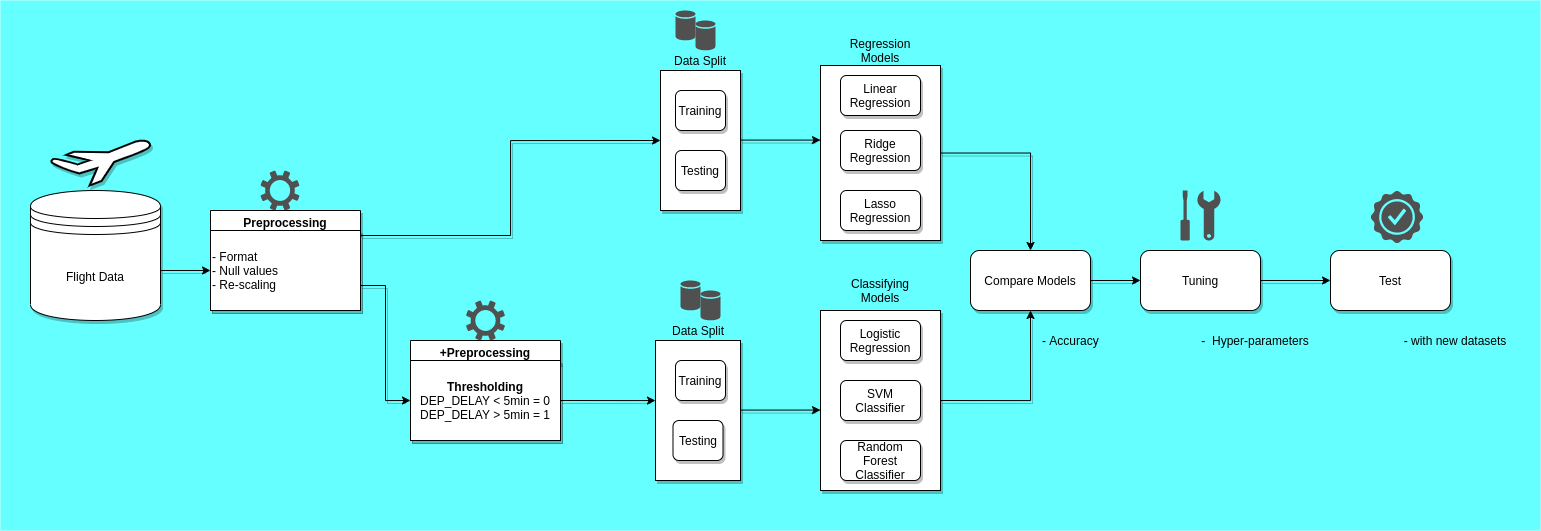
\includegraphics[clip, width=0.95\textwidth]{blockDiagram.png}
\caption{The Proposed Approach.}
\label{fig:app}
\end{figure*} 


\section{The Proposed Model}\label{Section III}

In statistics, linear regression is an approach for modeling the relationship between a scalar dependent variable Y and one or more explanatory variables (or independent variables) denoted X. The case of one explanatory variable is called simple linear regression. For more than one explanatory variable, the process is called multiple linear regression. In linear regression, the relationships are modeled using linear predictor functions whose unknown model parameters are estimated from the data. Such models are called linear models. Linear regression has many practical uses. Most applications fall into one of the following two broad categories: 
\begin{enumerate}
    
\item If the goal is prediction, or forecasting, or error reduction, linear regression can be used to fit a predictive model to an observed data set of Y and X values. After developing such a model, if an additional value of X is then given without its accompanying value of Y, the fitted model can be used to make a prediction of the value of Y. 
\item Given a variable Y and a number of variables X$_i$ and X$_p$ that may be related to Y, linear regression analysis can be applied to quantify the strength of the relationship between Y and the X$_j$, to assess which X$_j$ may have no relationship with Y at all, and to identify which subsets of the X$_j$ contain redundant information about Y.
\end{enumerate}
The decisions taken in the management of an airport are often based on common sense and influence several variables, such as flight delay. Reducing this delay presents the advantage of decreasing costs and increasing the quality of the service provided to the passengers. It is thus important to find which variables influence flight delay and use them to predict it. In this context, there are many studies. Some of them treat flight delay prediction as a regression problem, predicting the delay by the minute, and others as a classification problem, predicting a time interval where the delay will fall. The problem here considered is to predict flight arrival delay at a given airport. 

Given information about a flight that will depart from this airport, the main objective in this scope is to predict its arrival delay by the minute. If the delay time falls into a predefined range, it indicates that there is no delay in the flight. If the delay time falls above the range it indicates the flight delay. So, two types of prediction mechanisms are considered: regression, where the continuous output is an estimate of the arrival delay, and classification, where the output is a binary prediction of whether the arrival delay is more or less than the predefined threshold.

It is important to find which variables influence flight delay and use them to predict it. After careful analysis of the data, we found that there is a close relation between arrival delay and departure delay. So, we can use departure delay to predict arrival delay. Using the formula as given by Eq. \ref{eq1}.
\begin{equation}\label{eq1}
    Y=\beta_1X_1+\beta_2X_2+\beta_3
\end{equation}


We establish a multiple linear regression model , where the target variable Y is arrival delay, the predictor variables X$_1$ is departure delay and X$_2$ is route distance.

At first, we add a field of departure delay subtracting the planned departure time with the actual departure time. In the training phase, we use departure delay and route distance training model in order to learn the three parameters. In the predicting phase, given information about a flight that will depart from one airport, route distance is already known. If we know the departure delay of the flight, we could use the model to predict its arrival delay, so as to determine whether the flight delay. Given information about a flight, at first, we look for the similar data according to the departure airport, the aircraft type and the weather of departure airport in the dataset, and then we cluster the similar data using departure delay and set up a threshold. If the amount of data exceeds the threshold, we calculate the average of departure delay, and use it as the departure delay of the given flight.

After removing the outliers we ran the regression models again and we found out that the linear regression is the second best in terms of errors compared to the other regression. 

\begin{figure*} [!t]
\centering
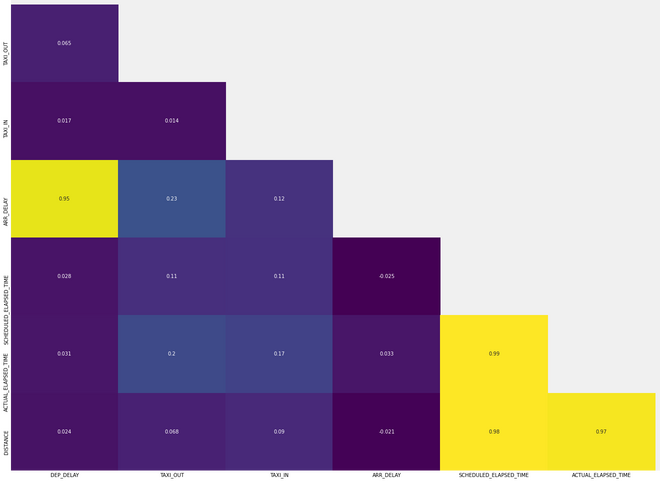
\includegraphics[clip, width=0.75\textwidth]{rsz_cleaned.png}
\caption{Correlation Heatmap with selected features and predict value.}
\label{fig:ch}
\end{figure*}  

%------------------------------------
\section{Experimental Analysis}\label{Section IV}
%-------------------------------------

\subsection{Dataset}\label{dataset}

\begin{enumerate}[label=\roman*.]
\item The original dataset contained 28 attributes out of which 3 were integers, 5 were strings, and 20 were floats. There were 5819079 entries. It contained dates, places, times and multiple types of delays. 
\item First and foremost, we made sure that the attributes had a general format and scale. Unwanted attributes such as ORIGIN and DEST, as well as all the attributes which had more than 80 percent of their entries missing such as the cancelled flights and diverted  flights were removed. One of the main problems while getting the dataset ready for the model was that the time formats in the original dataset, they were not properly formatted. To overcome this we had to create a function which would take the dates which were in float format and convert them into proper datetime format. Initially, for the final dataset after cleaning and preprocessing and using the correlation heatmap for the best attributes, we have:

\begin{enumerate}
\item DEP\_DELAY: Datetime format calculated as a difference between scheduled and actual delay
\item ARR\_DELAY: Datetime format calculated as a difference between scheduled and actual delay
\item SCHEDULED\_ELAPSED\_TIME: Datetime format which show the elapsed time for the flight taking the scheduled time into consideration
\item ACTUAL\_ELAPSED\_TIME: Datetime format which show the elapsed time for the flight that happened taking the delays into consideration
\item DISTANCE: An int datatype which shows total distance travelled in given elapsed time.
\end{enumerate}

The following 2 features were later added after using Random Forest Feature Selection:
\begin{enumerate}
\item TAXI\_IN: A float datatype that shows the time taken for the plane to reach the gate from the tarmac.
\item TAXI\_OUT: A float datatype that shows the time taken for the plane to reach the tarmac from the gate.
\end{enumerate} 
The correlation Heatmap with the features and the predict attribute can be seen in Fig.~\ref{fig:ch}.
\end{enumerate}

%----------****-----------------
\subsection{Experimental Setup}
%----------****-----------------
In order to perform the project, the following were the specifications of the software environment:
\begin{enumerate}[label=\roman*.]
\item
\begin{itemize}
\item[] Operating System: Windows 10 / Arch Linux
\item[]Development Language: Python3
\item[]Development Tool: Google Colab
\item[]Hardware: Python 3 Google Compute Backend
\item[]RAM: 12.72GB
\item[]Disk: 107.77GB
\end{itemize}

\item The initial testing with regression models was done without removing the outliers and also all the numeric features of the dataset were used. However, the later regression models were done with removal of outliers. Various trials were done taking features which were least correlated to highly correlated into consideration for better output of the regression model.
\end{enumerate}

\subsection{Results and Discussion}\label{recall}
We compared Linear Regression, Ridge Regression, Lasso Regression, Logistic Regression, SVM and Random Forest Classification. 

\renewcommand{\arraystretch}{1.5}
\begin{table}[h!]
\normalsize

\begin{tabular}{|c|c|c|c|}
\hline
\textbf{Models} & \textbf{Testing Score} & \textbf{RMSE} & \textbf{MAE} \\ \hline
\textbf{Linear Regression} & 0.499 & 0.313 & 0.207 \\ \hline
\textbf{Ridge Regression} & 0.323 & 0.364 & 0.307 \\ \hline
\textbf{Lasso Regression} & -2.67 & 0.442 & 0.391 \\ \hline
\end{tabular}
\caption{Performance Comparison: Linear Regression vs Ridge Regression vs Lasso Regression w.r.t. Testing score, Root Mean Square Error (RMSE) and Mean Absolute Error (MAE)}
\label{table:1}
\end{table}
As we can see from the Table \ref{table:1} regression models did not produce satisfactory results. They had very low testing  scores. To get better results we used the other regression models. Initially, running Logistic Regression on our model with 4 features and 1623633 data points, gives us an accuracy of around 0.6918. The stratified k fold cross validation was done with 5 folds. Also, initially running SVM gave much low accuracy of around 0.48 which is not good enough. Additionally, Random Forest Classifier received an accuracy of 0.69. i.e. the prediction of aircraft with delay is about 0.69 times. However, this accuracy will improve after some fine-tuning.
\\\\
After adding two more features into the models namely 'TAXI\_IN' and 'TAXI\_OUT' and increasing the data-set to 6000000 data-points the accuracy for each model was greatly improved(Table \ref{table:2}). For the Random Forest Classifier we also did rigorous hyper parameter tuning using RandomizedSearchCV() and GridSearchCV() to get the optimal hyperparameters. Doing so resulted in an accuracy of 0.862015 for Random Forest Classifier. The table shows new accuracy after making those changes.
\\\\
Comparing the accuracy of the three methods accuracy rates(table \ref{table:2}), Random Forest Classifier proves to be the leading model. Also, the confusion matrices of Logistic Regression (Table \ref{table:3}), SVM (Table \ref{table:4}), and Random Forest (Table \ref{table:5}) are given below.
 
\begin{table}[h!]
\begin{tabular}{|l|l|l|l|l|}
\hline
\normalsize
\textbf{Model} & \textbf{Accuracy} & \textbf{Sensitivity} & \textbf{Specificity} & \textbf{PPV} \\ \hline
\textbf{LR}&  85.72\%. &75.40\%.  & 88.90\%. & 87.16\%. \\ \hline
\textbf{SVM} & 71.77\%. & 7.90\%. & 93.10\%. & 53.37\%. \\ \hline
\textbf{RF} & 86.20\%. & 75.80\%. & 86.50\%. &  84.88\%.\\ \hline
\end{tabular}
\caption{Performance Comparison: Logistic Regression (LR) vs SVM Classifier  vs Random Forest Classifier (RF) w.r.t. Accuracy, Sensitivity and Positive Predictive Value (PPV)}
\label{table:2}
\end{table}

\begin{table}[h!]
\normalsize
\begin{tabular}{|c|c|}
\hline
\begin{tabular}[c]{@{}c@{}}True Negative\\ 88.9\%.\end{tabular} & \begin{tabular}[c]{@{}c@{}}False Positive\\ 11.1\%.\end{tabular} \\ \hline
\begin{tabular}[c]{@{}c@{}}False Negative\\ 24.6\%.\end{tabular} & \begin{tabular}[c]{@{}c@{}}True Positive\\ 75.4\%.\end{tabular} \\ \hline
\end{tabular}
\caption{Logistic Regression results w.r.t. Confusion Matrix}
\label{table:3}
\end{table}

\begin{table}[H]
\normalsize
\begin{tabular}{|c|c|}
\hline
\begin{tabular}[c]{@{}c@{}}True Negative\\ 93.1\%.\end{tabular} & \begin{tabular}[c]{@{}c@{}}False Positive\\ 6.9\%.\end{tabular} \\ \hline
\begin{tabular}[c]{@{}c@{}}False Negative\\ 92.1\%.\end{tabular} & \begin{tabular}[c]{@{}c@{}}True Positive\\ 7.9\%.\end{tabular} \\ \hline
\end{tabular}
\caption{SVM results w.r.t. Confusion Matrix}
\label{table:4}
\end{table}

\begin{table}[h!]
\normalsize
\begin{tabular}{|c|c|}
\hline
\begin{tabular}[c]{@{}c@{}}True Negative\\ 86.5\%.\end{tabular} & \begin{tabular}[c]{@{}c@{}}False Positive\\ 13.5\%.\end{tabular} \\ \hline
\begin{tabular}[c]{@{}c@{}}False Negative\\ 24.2\%.\end{tabular} & \begin{tabular}[c]{@{}c@{}}True Positive\\ 75.8\%.\end{tabular} \\ \hline
\end{tabular}
\caption{Random Forest Classifier results w.r.t. Confusion Matrix}
\label{table:5}
\end{table}

If there were more influencing factors such as weather and wind direction our model would have potentially improved its  accuracy. These types of impact changing factors are discussed in  “Predicting Airline Delays”[\ref{[11]}] and “Multi-Factor Model for Predicting Delay at U.S. Airports”[\ref{[10]}].

Threshold of 5 minutes was defined for DEP\_DELAY and ARR\_DELAY attributes. If the DEP\_DELAY was less than or equal to 5 minutes then it was considered ‘0’ and if it was more than 5 minutes it was considered as ‘1’. Doing so resulted in making our problem a classification problem. 

However, after performing the operation it was seen that there was a vast difference between no. of attributes that were ‘0’ and the number of attributes that were ‘1’. Thus, to overcome this skewed attribute problem we selected only an equal number of ‘1’ and ‘0’ attributes as it has in the main data-set with the same ration(75:25) and merged into one data-set and used that to split our data-set into training and testing. Thus eliminating the skewed data-set problem.

Our model can also be used to make predictions for specific kinds of delays. For example there are different types of delays like weather delay, delay due to incoming air traffic.
We can also run these classification models for predicting those delays.
  
Overfitting happened for SVM and was resolved by tuning hyperparameter MAX\_Iteration. At first the Max\_Iteration was set to default which generated very low accuracy. After which there increments were made in 50 steps which resulted in overfitting at Max\_Iteration = 150. However, at lower iteration levels the SVM generated better True Negative and True Positives.

\section{Conclusion}\label{Section V}
 

This paper proposes an airline-delay prediction model using random forest classifier. From the examination performed on the data-set, we can presume that the factors which were incorporated in airline delay are ultimately affected via air-traffic. Thus, if there is a shift in air-traffic, delay times  would be influenced and be changed. Airline Carriers have most traffic when they have high-recurrence of flights.

The accuracy of 86\%. for the model was achieved by optimizing the hyper parameters for Random Forest Classifier, using randomized search to get an approximate of best parameters. Afterwards we get that we an exhaustive grid search which then tries every single possible combination of the hyper parameters. The model parameters that were used to achieve the accuracy are bootstrap=True, max\_.depth = 10, max\_.features= 2, min\_.samples\_.leaf= 4, min\_.samples\_.split= 2, n\_.estimators= 400. A disadvantage for using this is the trade off with time with every additional parameters and cross-validation that we add. The functions that we ran took a long amount of time to compute since it was a large dataset.    
 

\section*{Acknowledgements}\label{Acknowledgements}
\begin{center}
This work acknowledges The U.S. Department of Transportation's (DOT) Bureau of Transportation Statistics, the organizer of the Airline Data-set and Dr. Thangarajah Akilan for the technical comments and suggestions.
\end{center}

\section*{}\label{Refrences}
\begingroup 
\fontsize{8pt}{10pt}
\begin{thebibliography}{00} 
\bibitem{b1}\label{[1])}Beatty, R. Hsu, L. Berry, \&. J. Rome, “Preliminary evaluation of flight delay propagation through an airline schedule. 2nd USA/Europe Air Traffic Management R\&.D Seminar,” 7(4):259–270, 1998.
\bibitem{b2}\label{[2]}D. Markovic, T. Hauf, P. Rohner, \&. U. Spehr.,"A statistical study of the weather impact ¨ on punctuality at Frankfurt airport. Meteorological Applications,"15(2):293–303, 2008.
\bibitem{b3}\label{[3]}J. Xiong \&.  M. Hansen,"Modelling airline flight cancellation decisions. Transportation Research Part E: Logistics \&.Transportation Review," 56(Supplement C):64–80, Sept. 2013.
\bibitem{b4}\label{[4]} L. Hao, M. Hansen, Y. Zhang, \&. J. Post,"New York, New York: Two ways of estimating the delay impact of New York airports. Transportation Research Part E: Logistics and Transportation Review",70(Supplement C):245–260, Oct. 2014.
\bibitem{b5}\label{[5]} M. Abdel-Aty, C. Lee, Y. Bai, X. Li, and M. Michalak, "Detecting periodic patterns of arrival delay. Journal of Air Transport Management", 13(6):355–361, Nov. 2007. 
\bibitem{b6}\label{[6]}Y. Tu, M. O. Ball, and W. S. Jank, "Estimating flight departure delay distributions—a statistical approach with long-term trend and short-term pattern. Journal of the American Statistical Association", 103(481):112–125, 2008.
\bibitem{b7}\label{[7]}T. Kotegawa, D. De Laurentis, K. Noonan, and J. Post. "Impact of commercial airline network evolution on the U.S. air transportation system. In Proceedings of the 9th USA/Europe Air Traffic Management Research and Development Seminar", ATM 2011, pages 572–580, 2011.
\bibitem{b8} \label{[8]}S. AhmadBeigi, A. Cohn, Y. Guan, and P. Belobaba," Analysis of the potential for delay propagation in passenger airline networks. Journal of Air Transport Management", 14(5):221–236, Sept. 2008.
\bibitem{b9} \label{[9]}N. Xu, G. Donohue, K. B. Laskey, and C.-H. Chen, "Estimation of delay propagation in the national aviation system using Bayesian networks. In 6th USA/Europe Air Traffic Management Research and Development Seminar", Citeseer, 2005. 
\bibitem{b10}\label{[10]} Xu, Sherry, \& Laskey, 2008, "Multi-Factor Model for Predicting Delays at
U.S. Airports", "http://catsr.ite.gmu.edu/pubs/XuMultiFactorModelAirpor
tDelays
TRBv6.pdf"
\bibitem{b11} \label{[11]}Bandyopadhyay \&. Guerrero, 2012,"Predicting Airline Delays", http://cs229.stanford.edu/proj2012/BandyopadhyayGuerrero-PredictingFlightDelays\.pdf
\bibitem{b12}\label{[12]}W.-W. Wu, T.-T. Meng, and H.-Y. Zhang, "Flight plan optimization based on airport delay prediction. Jiaotong Yunshu Xitong Gongcheng Yu Xinxi/Journal of Transportation Systems Engineering and Information Technology", 16(6):189–195, 2016.
\bibitem{b13}\label{[13]}J. J. Rebollo and H. Balakrishnan," Characterization and prediction of air traffic delays. Transportation Research Part C: Emerging Technologies", 44(Supplement C):231–241, July 2014. 
\bibitem{b14}\label{[14]}P. Balakrishna, R. Ganesan, and L. Sherry," Accuracy of reinforcement learning algorithms for predicting aircraft taxi-out times: A case-study of Tampa Bay departures. Transportation Research Part C: Emerging Technologies", 18(6):950–962, Dec. 2010.
\bibitem{b15}\label{[15]}P. Balakrishna, R. Ganesan, L. Sherry, and B. S. Levy,"Estimating Taxi-out times with a reinforcement learning algorithm. In 2008 IEEE/AIAA 27th Digital Avionics Systems Conference", pages 3.D.3–1–3.D.3–12, Oct. 2008.

\bibitem{b16}\label{[16]}L. Zonglei, W. Jiandong, and Z. Guansheng, "A New Method to Alarm Large Scale of Flights Delay Based on Machine Learning. In 2008 International Symposium on Knowledge Acquisition and Modeling", pages 589–592, Dec. 2008
\end{thebibliography} 
\endgroup 

\end{document}
